\documentclass[12pt,a4paper]{article}         %% typ dokumentu

\usepackage{amsmath,amsfonts,amssymb}   %% makra
\usepackage[czech]{babel}
\usepackage[utf8]{inputenc}
\usepackage{bold-extra}
\usepackage{tikz}
\usepackage{circuitikz}
    \usetikzlibrary{arrows}
\usepackage{float}
\usepackage{graphicx}
\usepackage{textcomp}
\usepackage{caption}



\newcommand{\prvniZadani}[1]{
        \def\prvniSkupina{#1}
        Stanovte napětí $U_{R5}$ a proud $I_{R5}$. Použijte metodu postupného zjednodušování obvodu. \\
        
        \begin{tabular}{|c|c|c|c|c|c|c|c|c|c|c|} \hline
sk. & $U_1$ [\Vo] & $U_2$ [\Vo]  & $R_1$ [$\Omega$] & $R_2$ [$\Omega$] & $R_3$ [$\Omega$] & $R_4$ [$\Omega$] & $R_5$ [$\Omega$] & $R_6$ [$\Omega$] & $R_7$ [$\Omega$] & $R_8$ [$\Omega$] \\ \hline
    \ifthenelse{\equal{#1}{A}}
    {A & 80 & 120 & 350 & 650 & 410 & 130 & 360 & 750 & 310 & 190}{}
    \ifthenelse{\equal{#1}{B}}
    {B & 95 & 115 & 650 & 730 & 340 & 330 & 410 & 830 & 340 & 220}{}
    \ifthenelse{\equal{#1}{C}}
    {C & 100 & 80 & 450 & 810 & 190 & 220 & 220 & 720 & 260 & 180}{}
    \ifthenelse{\equal{#1}{D}}
    {D & 105 & 85 & 420 & 980 & 330 & 280 & 310 & 710 & 240 & 200}{}
    \ifthenelse{\equal{#1}{E}}
    {E & 115 & 55 & 485 & 660 & 100 & 340 & 575 & 815 & 255 & 225}{}
    \ifthenelse{\equal{#1}{F}}
    {F & 125 & 65 & 510 & 500 & 550 & 250 & 300 & 800 & 330 & 250}{}
    \ifthenelse{\equal{#1}{G}}
    {G & 130 & 60 & 380 & 420 & 330 & 440 & 450 & 650 & 410 & 275}{}
    \ifthenelse{\equal{#1}{H}}
    {H & 135 & 80 & 680 & 600 & 260 & 310 & 575 & 870 & 355 & 265}{}
    \\ \hline \end{tabular} \\
    
    \includegraphics[scale=0.5,keepaspectratio]{fig/Pr1_2019.pdf} \\ 
    }
        
    % druhy priklad
    \newcommand{\druhyZadani}[1]{
        \def\druhySkupina{#1}
        Stanovte napětí $U_{R6}$ a proud $I_{R6}$. Použijte metodu Théveninovy věty. \\
        
         \begin{tabular}{|c|c|c|c|c|c|c|c|c|} \hline
sk. & $U$ [\Vo] & $R_1$ [$\Omega$] & $R_2$ [$\Omega$] & $R_3$ [$\Omega$] & $R_4$ [$\Omega$] & $R_5$ [$\Omega$] & $R_6$ [$\Omega$] \\ \hline
    \ifthenelse{\equal{#1}{A}}
    {A & 50 & 100 & 525 & 620 & 210 & 530 & 100}{}
    \ifthenelse{\equal{#1}{B}}
    {B & 100 & 50 & 310 & 610 & 220 &  570 & 200}{}
    \ifthenelse{\equal{#1}{C}}
    {C & 200 & 70 & 220 & 630 & 240 & 450 & 300}{}
    \ifthenelse{\equal{#1}{D}}
    {D & 150 & 200 & 200 & 660 & 200 & 550 & 400}{}
    \ifthenelse{\equal{#1}{E}}
    {E & 250 & 150 & 335 & 625 & 245 & 600 & 150}{}
    \ifthenelse{\equal{#1}{F}}
    {F & 130 & 180 &350 & 600 & 195 & 650 & 250}{}
    \ifthenelse{\equal{#1}{G}}
    {G & 180 & 250 & 315 & 615 & 180 & 460 & 350}{}
    \ifthenelse{\equal{#1}{H}}
    {H & 220 & 190 & 360 & 580 & 205 & 560 & 180}{}
    \\ \hline \end{tabular} \\
    
    \includegraphics[scale=0.5,keepaspectratio]{fig/Pr2_2019.pdf} \\
    }

    % treti priklad
    \newcommand{\tretiZadani}[1]{
        \def\tretiSkupina{#1}
        Stanovte napětí $U_{R4}$ a proud $I_{R4}$. Použijte metodu uzlových napětí ($U_A$, $U_B$, $U_C$). 
        
        \begin{tabular}{|c|c|c|c|c|c|c|c|c|} \hline
sk. & $U$ [\Vo] & $I_1$ [\Am] & $I_2$ [\Am] & $R_1$ [$\Omega$] & $R_2$ [$\Omega$] & $R_3$ [$\Omega$] & $R_4$ [$\Omega$] & $R_5$ [$\Omega$] \\ \hline
    \ifthenelse{\equal{#1}{A}}
    {A & 120 & 0.9  & 0.7  & 53 & 49 & 65 & 39 & 32}{}
    \ifthenelse{\equal{#1}{B}}
    {B & 150 & 0.7  & 0.8  & 49 & 45 & 61 & 34 & 34}{}
    \ifthenelse{\equal{#1}{C}}
    {C & 110 & 0.85 & 0.75 & 44 & 31 & 56 & 20 & 30}{}
    \ifthenelse{\equal{#1}{D}}
    {D & 115 & 0.6  & 0.9  & 50 & 38 & 48 & 37 & 28}{}
    \ifthenelse{\equal{#1}{E}}
    {E & 135 & 0.55 & 0.65 & 52 & 42 & 52 & 42 & 21}{}
    \ifthenelse{\equal{#1}{F}}
    {F & 145 & 0.75 & 0.85 & 48 & 44 & 53 & 36 & 25}{}
    \ifthenelse{\equal{#1}{G}}
    {G & 160 & 0.65 & 0.45 & 46 & 41 & 53 & 33 & 29}{}
    \ifthenelse{\equal{#1}{H}}
    {H & 130 & 0.95 & 0.50 & 47 & 39 & 58 & 28 & 25}{}
    \\ \hline \end{tabular} \\
    
    \includegraphics[scale=0.5,keepaspectratio]{fig/Pr3_2019.pdf} \\
    }
    
    % ctvrty  priklad
    \newcommand{\ctvrtyZadani}[1]{
        \def\ctvrtySkupina{#1}
        Pro napájecí napětí platí: $u_1=U_1{\cdot}\sin(2{\pi}ft)$, $u_2=U_2{\cdot}\sin(2{\pi}ft)$.\\
Ve vztahu pro napětí $u_{C_{2}}=U_{C_2}{\cdot}\sin(2{\pi}ft+\varphi_{C_{2}})$
určete $|U_{C_{2}}|$ a $\varphi_{C_{2}}$. Použijte metodu smyčkových proudů.\\

Pozn: Pomocné směry šipek napájecích zdrojů platí pro speciální časový okamžik ($t=\frac{\pi}{2{\omega}}$).
        
        \begin{tabular}{|c|c|c|c|c|c|c|c|c|c|} \hline
sk. & $U_1$ [\Vo] & $U_2$ [\Vo] & $R_1$ [$\Omega$] & $R_2$ [$\Omega$] & $L_{1}$ [\mH] & $L_{2}$ [\mH] & $C_1$ [$\uF$] & $C_2$ [$\uF$] & $f$ [\Hz] \\ \hline
    \ifthenelse{\equal{#1}{A}}
    {A & 35 & 55 & 12 & 14 & 120 & 100 & 200 & 105 & 70}{}
    \ifthenelse{\equal{#1}{B}}
    {B & 25 & 40 & 11 & 15 & 100 &  85 & 220 &  95 & 80}{}
    \ifthenelse{\equal{#1}{C}}
    {C & 35 & 45 & 10 & 13 & 220 &  70 & 230 &  85 & 75}{}
    \ifthenelse{\equal{#1}{D}}
    {D & 45 & 50 & 13 & 15 & 180 &  90 & 210 &  75 & 85}{}
    \ifthenelse{\equal{#1}{E}}
    {E & 50 & 30 & 14 & 13 & 130 &  60 & 100 &  65 & 90}{}
    \ifthenelse{\equal{#1}{F}}
    {F & 20 & 35 & 12 & 10 & 170 &  80 & 150 &  90 & 65}{}
    \ifthenelse{\equal{#1}{G}}
    {G & 55 & 50 & 13 & 12 & 140 &  60 & 160 &  80 & 60}{}
    \ifthenelse{\equal{#1}{H}}
    {H & 65 & 60 & 10 & 10 & 160 &  75 & 155 &  70 & 95}{}
    \\ \hline \end{tabular} \\
    \includegraphics[scale=0.5,keepaspectratio]{fig/Pr4_2019.pdf} \\
    }

    % paty priklad
    \newcommand{\patyZadani}[1]{
        \def\patySkupina{#1}
        V obvodu na obrázku níže v čase $t=0 $[s] sepne spínač $S$. Sestavte diferenciální rovnici popisující chování obvodu na obrázku, dále ji upravte dosazením hodnot parametrů. Vypočítejte analytické řešení
$u_{C}~=~f(t)$. Proveďte kontrolu výpočtu dosazením do sestavené diferenciální rovnice.\\

Pozn: Pomocné směry šipek napájecích zdrojů platí pro speciální časový okamžik ($t=\frac{\pi}{2{\omega}}$).\\
        
        \begin{tabular}{|c|c|c|c|c|} \hline
        sk. & $U$ [\Vo] & $C$ [F] & $R$ [$\Omega$] & $u_C(0)$ [\Vo] \\ \hline
    \ifthenelse{\equal{#1}{A}}
    {A & 40 & 50 & 10 & 16}{}
    \ifthenelse{\equal{#1}{B}}
    {B & 30 & 10 & 20 & 15}{}
    \ifthenelse{\equal{#1}{C}}
    {C & 35 & 5 & 30 & 14}{}
    \ifthenelse{\equal{#1}{D}}
    {D & 25 & 5 & 25 & 12}{}
    \ifthenelse{\equal{#1}{E}}
    {E & 40 & 30 & 40 & 11}{}
    \ifthenelse{\equal{#1}{F}}
    {F & 22 & 30 & 15 & 10}{}
    \ifthenelse{\equal{#1}{G}}
    {G & 20 & 50 & 25 & 8}{}
    \ifthenelse{\equal{#1}{H}}
    {H & 18 & 50 & 40 & 5}{}
    \\ \hline \end{tabular} \\
    \includegraphics[scale=0.5,keepaspectratio]{fig/Pr5_2019.pdf} \\
    }


%%%%%%%%%%%%%%%%%%%%%%%%%%%%%%%%%%%%%%%%%%%%%%% Dokument

\begin{document}
    %%%%%%%%%%%%%%%%%%%%%%%%%%%%%%%%%%%%%%%%%%%%%%% Titulní list 
    \begin{titlepage}
        \begin{center}
        	\textsc{\LARGE Vysoké Učení Technické v Brně}
        	    \\[0.5cm]
        	    {\LARGE Fakulta informačních technologií}
        
        	\vspace{6cm}
        
        	\textsc{\LARGE Elektronika pro informační technologie}
        	    \\[0.6cm]
                \textsc{\LARGE 2019/2020}
                \\[4cm]
                \textbf{\textsc{\LARGE Semestrální projekt}}
        \end{center}
        
        \vfill
        
        \begin{flushleft}
        	Karel Jirgl (xjirgl01)
        	\hfill
        	Brno, \today
        \end{flushleft}
    \end{titlepage}

    %%%%%%%%%%%%%%%%%%%%%%%%%%%%%%%%%%%%%%%%%%%%%%% Příklad 1
    \section*{1. - H \\
    Stanovte napětí UR5 a proud IR5. Použijte metodu postupného zjednodušování obvodu.}

 \begin{tabular}{|c|c|c|c|c|c|c|c|c|c|c|} \hline
sk. & $U_1$ [V] & $U_2$ [V]  & $R_1$ [$\Omega$] & $R_2$ [$\Omega$] & $R_3$ [$\Omega$] & $R_4$ [$\Omega$] & $R_5$ [$\Omega$] & $R_6$ [$\Omega$] & $R_7$ [$\Omega$] & $R_8$ [$\Omega$] \\ \hline

    {H & 135 & 80 & 680 & 600 & 260 & 310 & 575 & 870 & 355 & 265}{}
    
    \\ \hline \end{tabular} \\

    \begin{figure}[H] 
		\vspace{0cm}
		\center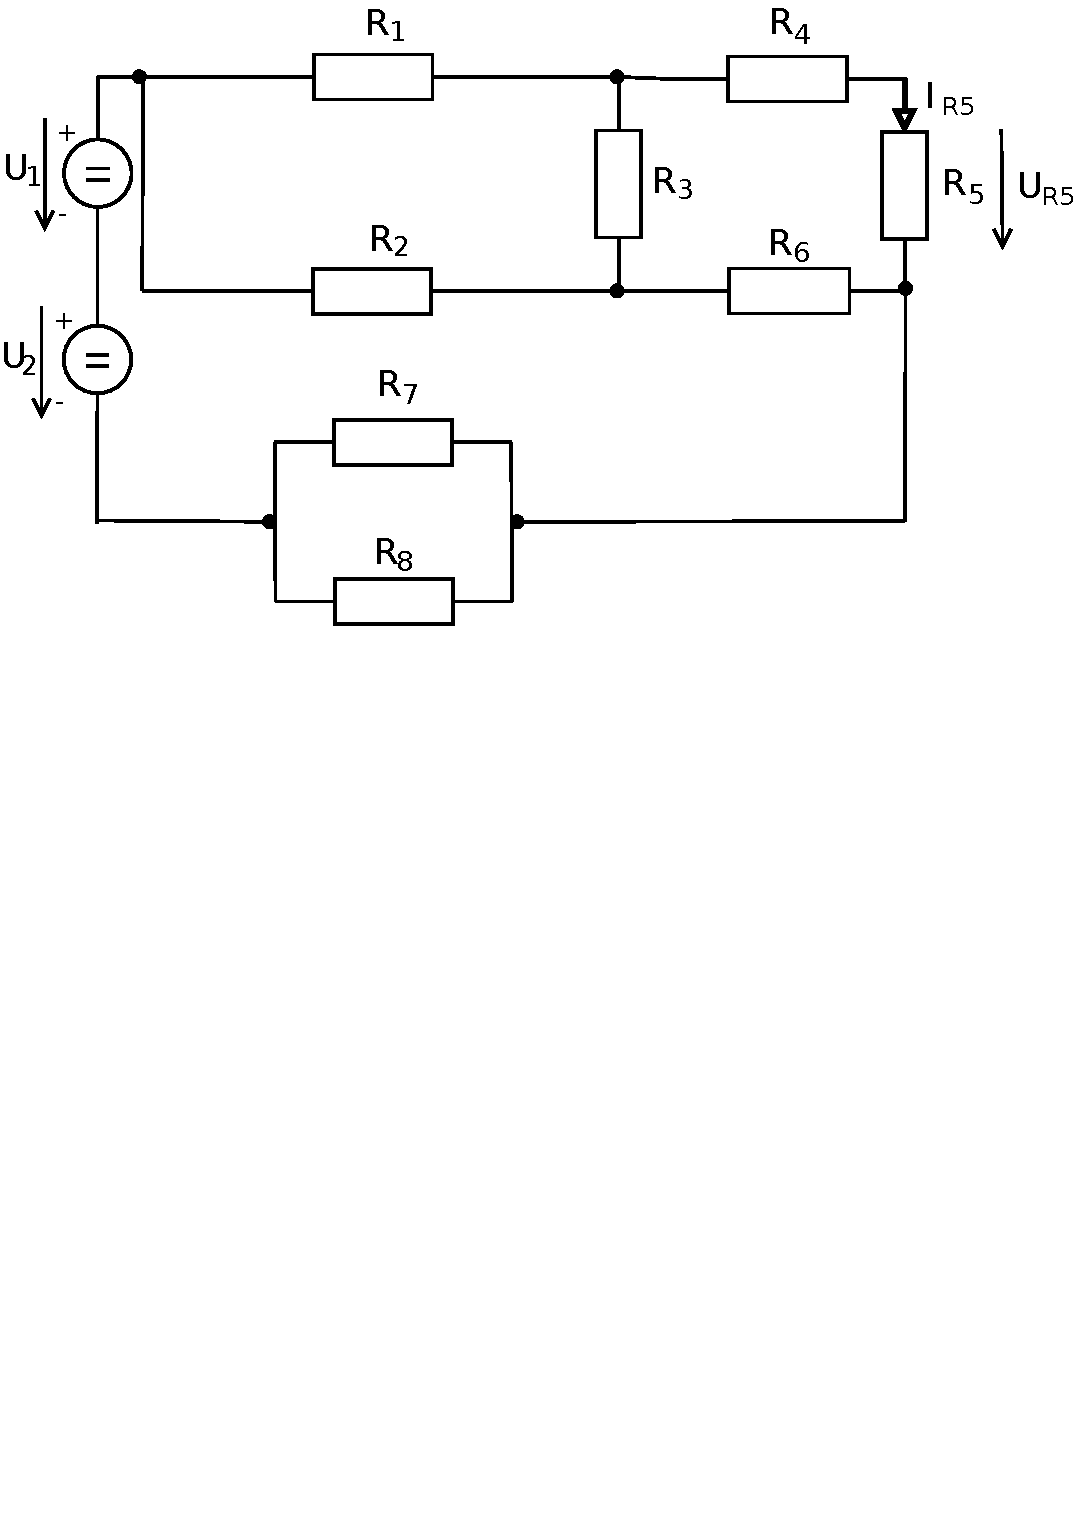
\includegraphics[trim={0 15cm 0 0},clip,width=0.6\linewidth]{obr/1_1}
		\caption*{Zadání}
    \end{figure}

    \begin{figure}[H] 
		\vspace{-0.6cm}
		\center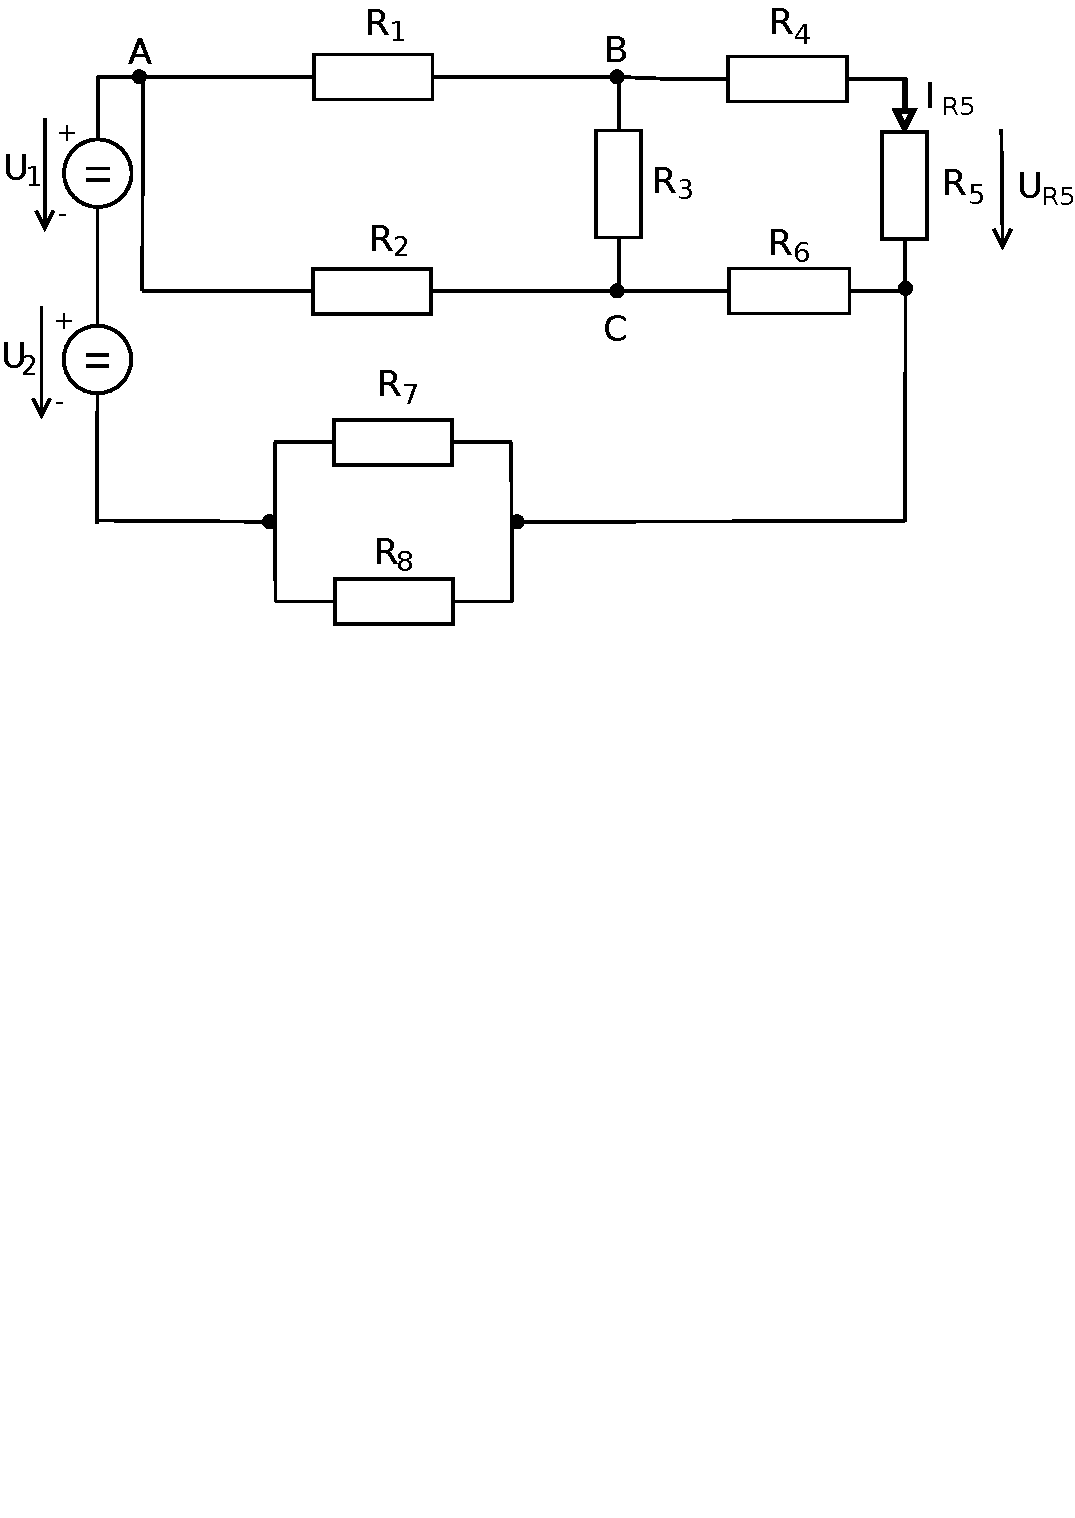
\includegraphics[trim={0 15cm 0 0},clip,width=0.6\linewidth]{obr/1_2}
		\caption*{Obvod postupně zjednodušujeme. Nejprve převedeme trojúhelník na hvězdu.}
    \end{figure}
    
    \newpage
    
    \begin{figure}[H] 
		\vspace{-0.6cm}
		\center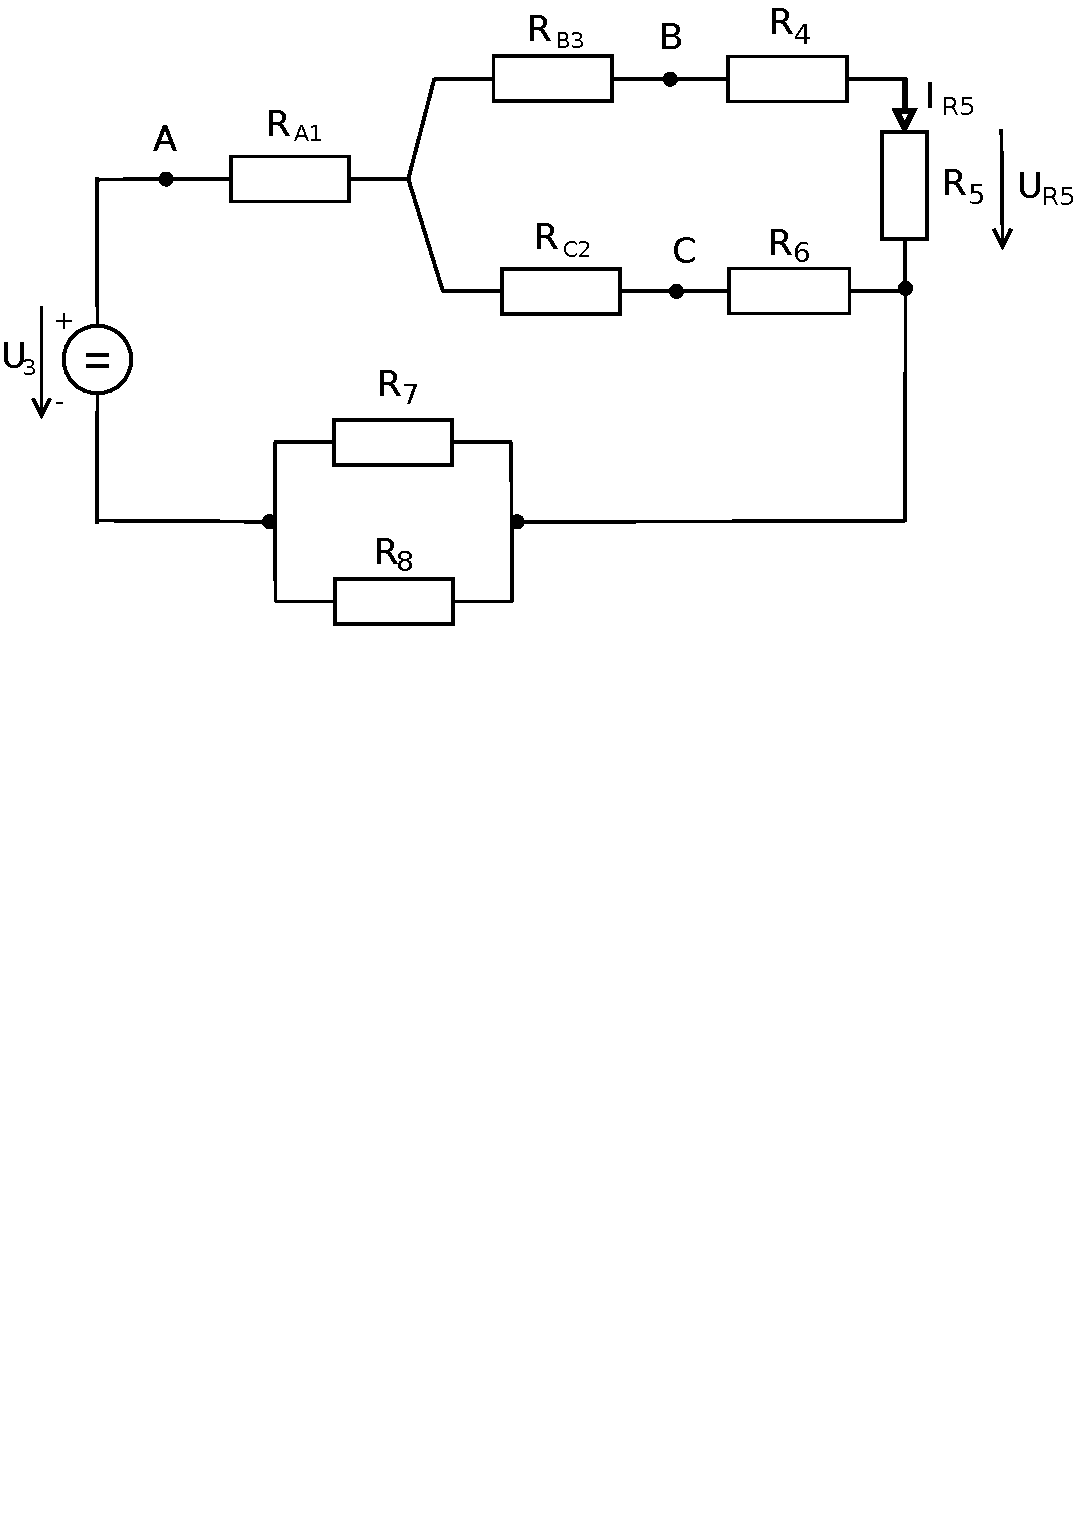
\includegraphics[trim={0 15cm 0 0},clip,width=0.7\linewidth]{obr/1_3}
    \end{figure}
    
    {\Large
        \begin{math}\\
        U_3 = U_1 + U_2 = 135 + 80 = 215 V\\
        R_D = \frac{R_7 \cdot R_8}{R_7 + R_8} = \frac{355 \cdot 265}{355 + 265} = 151,733871 {\Omega}\\
        \\
        R_A = R_{A1} = \frac{R_1 \cdot R_2}{R_1 + R_2 + R_3} = \frac{408000}{680 + 600 + 260} = 264,9350649 {\Omega}\\
        R_{B3} = \frac{R_1 \cdot R_3}{R_1 + R_2 + R_3} = \frac{176800}{1540} = 114,8051948 {\Omega}\\
        R_{C2} = \frac{R_2 \cdot R_3}{R_1 + R_2 + R_3} = \frac{156000}{1540} = 101,2987013 {\Omega}\\
        \end{math}
    }

    \begin{figure}[H] 
		\vspace{-0.6cm}
		\center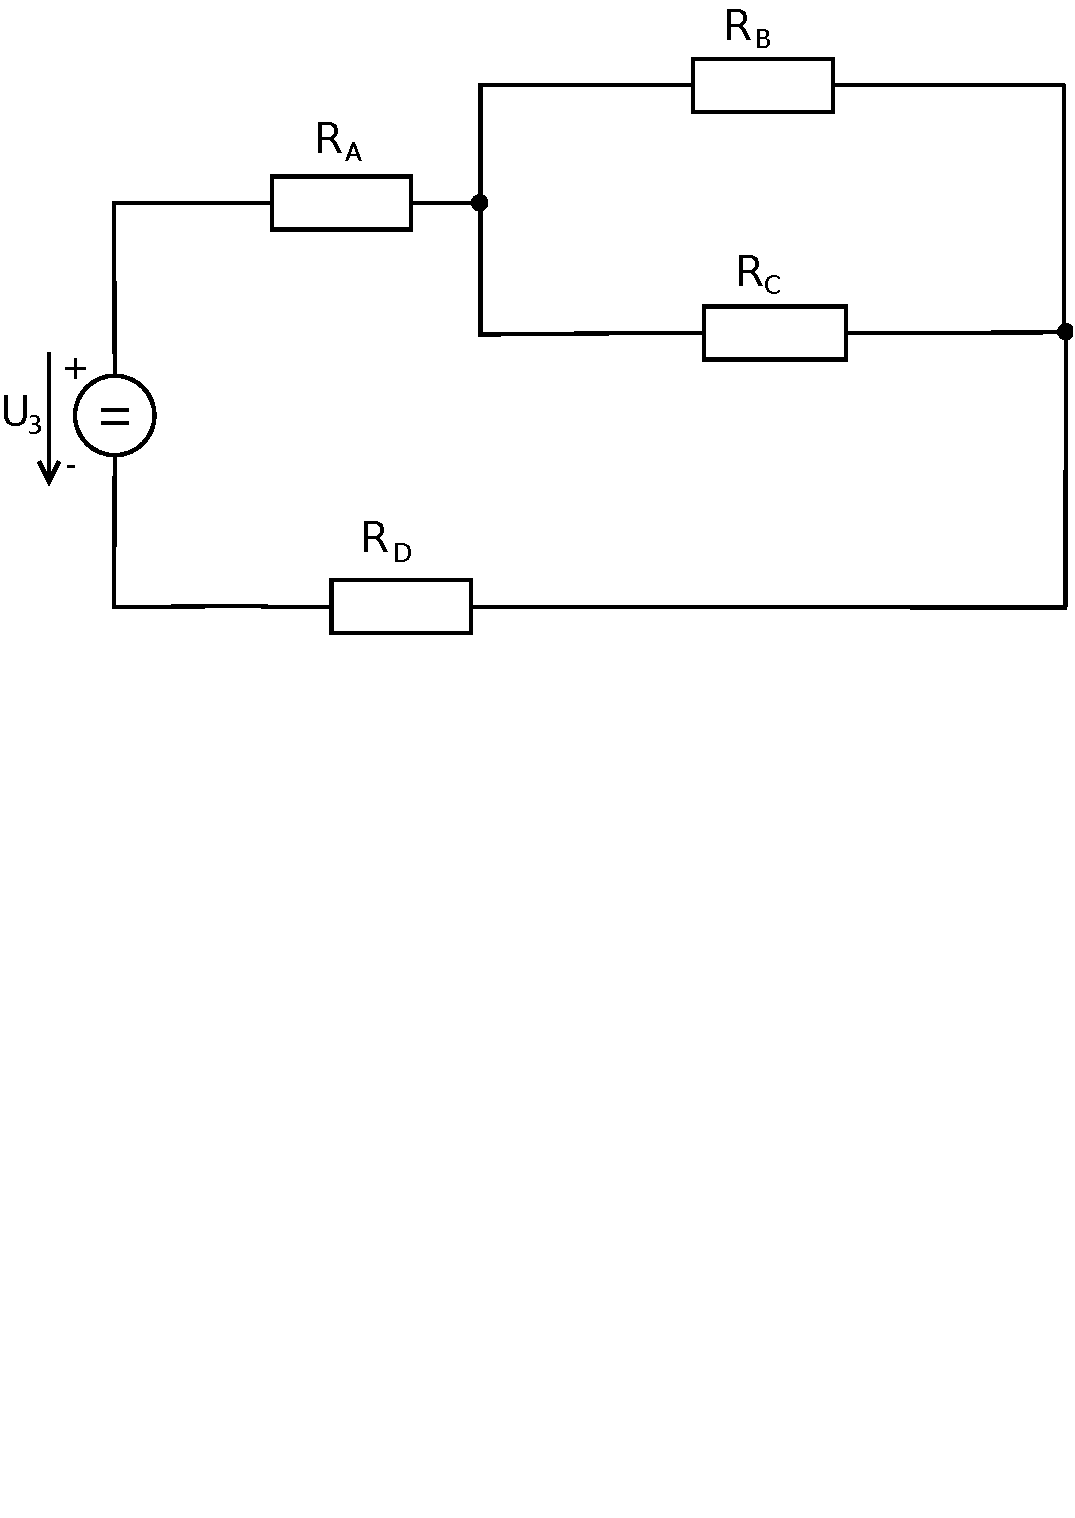
\includegraphics[trim={0 14cm 0 0},clip,width=0.6\linewidth]{obr/1_4}
    \end{figure}
    
    {\Large
        \begin{math}\\
        R_B = R_{B3} + R_4 +R_5 = 114,8052 + 310 + 575 = 999,8052 {\Omega}\\
        R_C = R_{C2} + R_6 = 101,2987 + 870 = 971,2987 {\Omega}\\
        \end{math}
    }

    
    \begin{figure}[H] 
		\vspace{-0.6cm}
		\center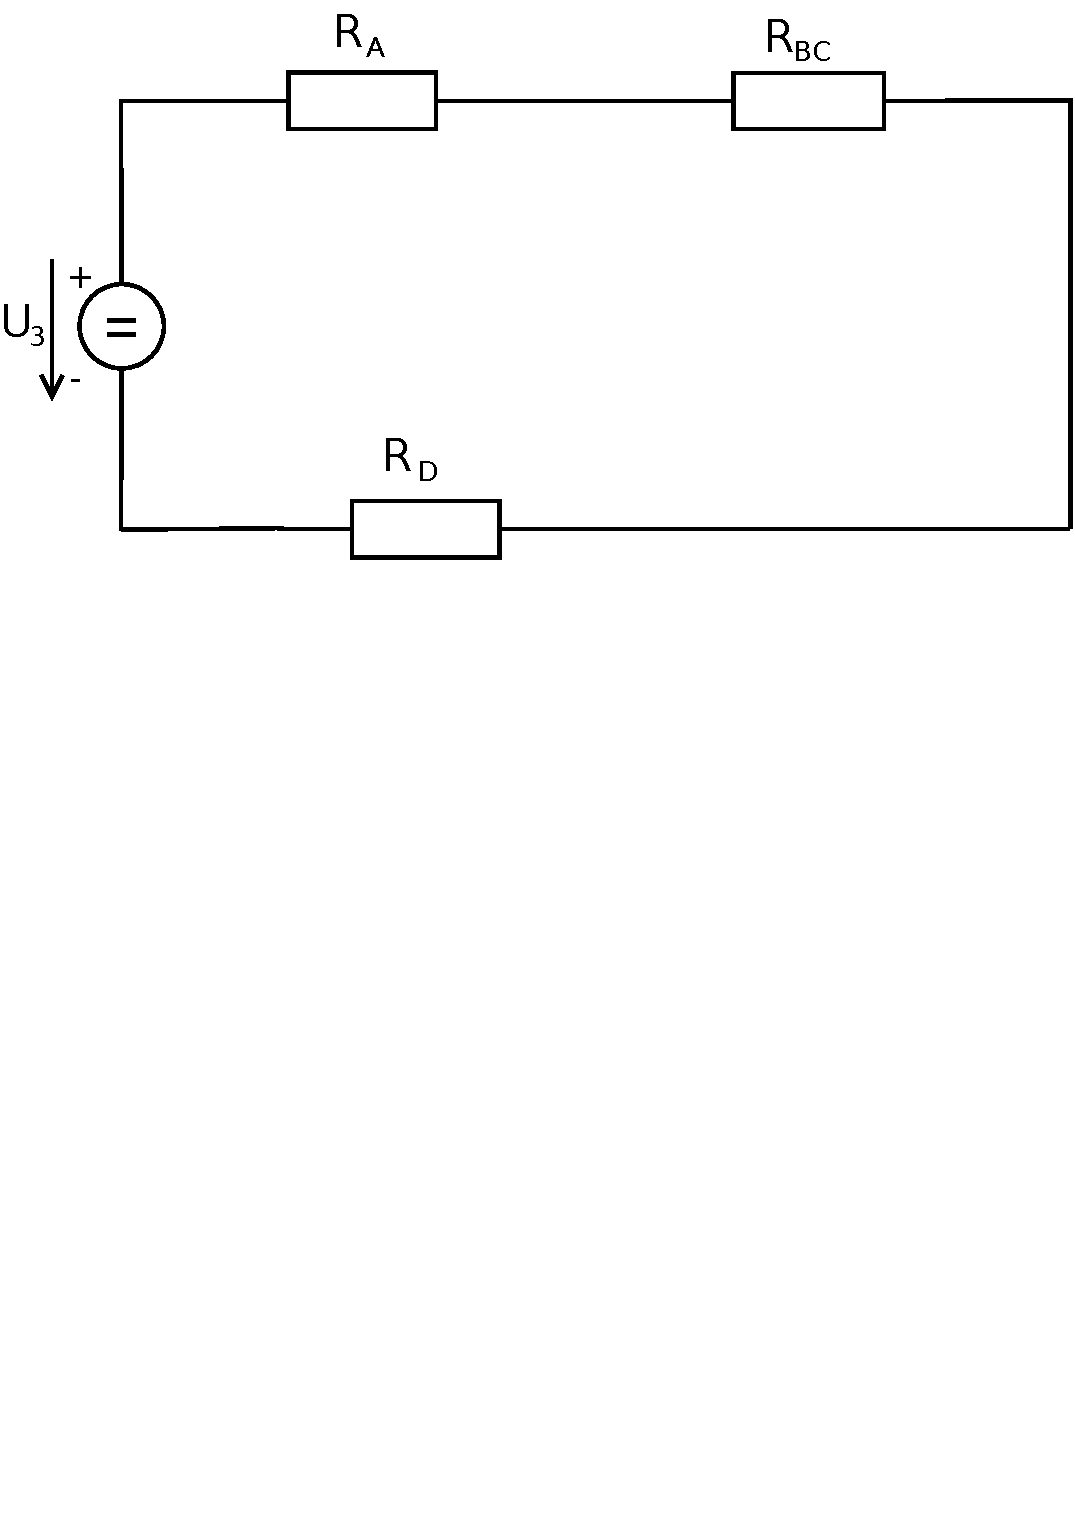
\includegraphics[trim={0 14cm 0 0},clip,width=0.6\linewidth]{obr/1_5}
    \end{figure}
    
    {\Large
        \begin{math}\\
        R_{BC} = \frac{R_B \cdot R_C}{R_B + R_C} = \frac{999,8052 \cdot 971,2987}{999,8052 + 971,2987} = \frac{971115,453}{1971,11} = 492,67 {\Omega}\\
        \end{math}
    }
    
    \begin{figure}[H] 
		\vspace{-0.6cm}
		\center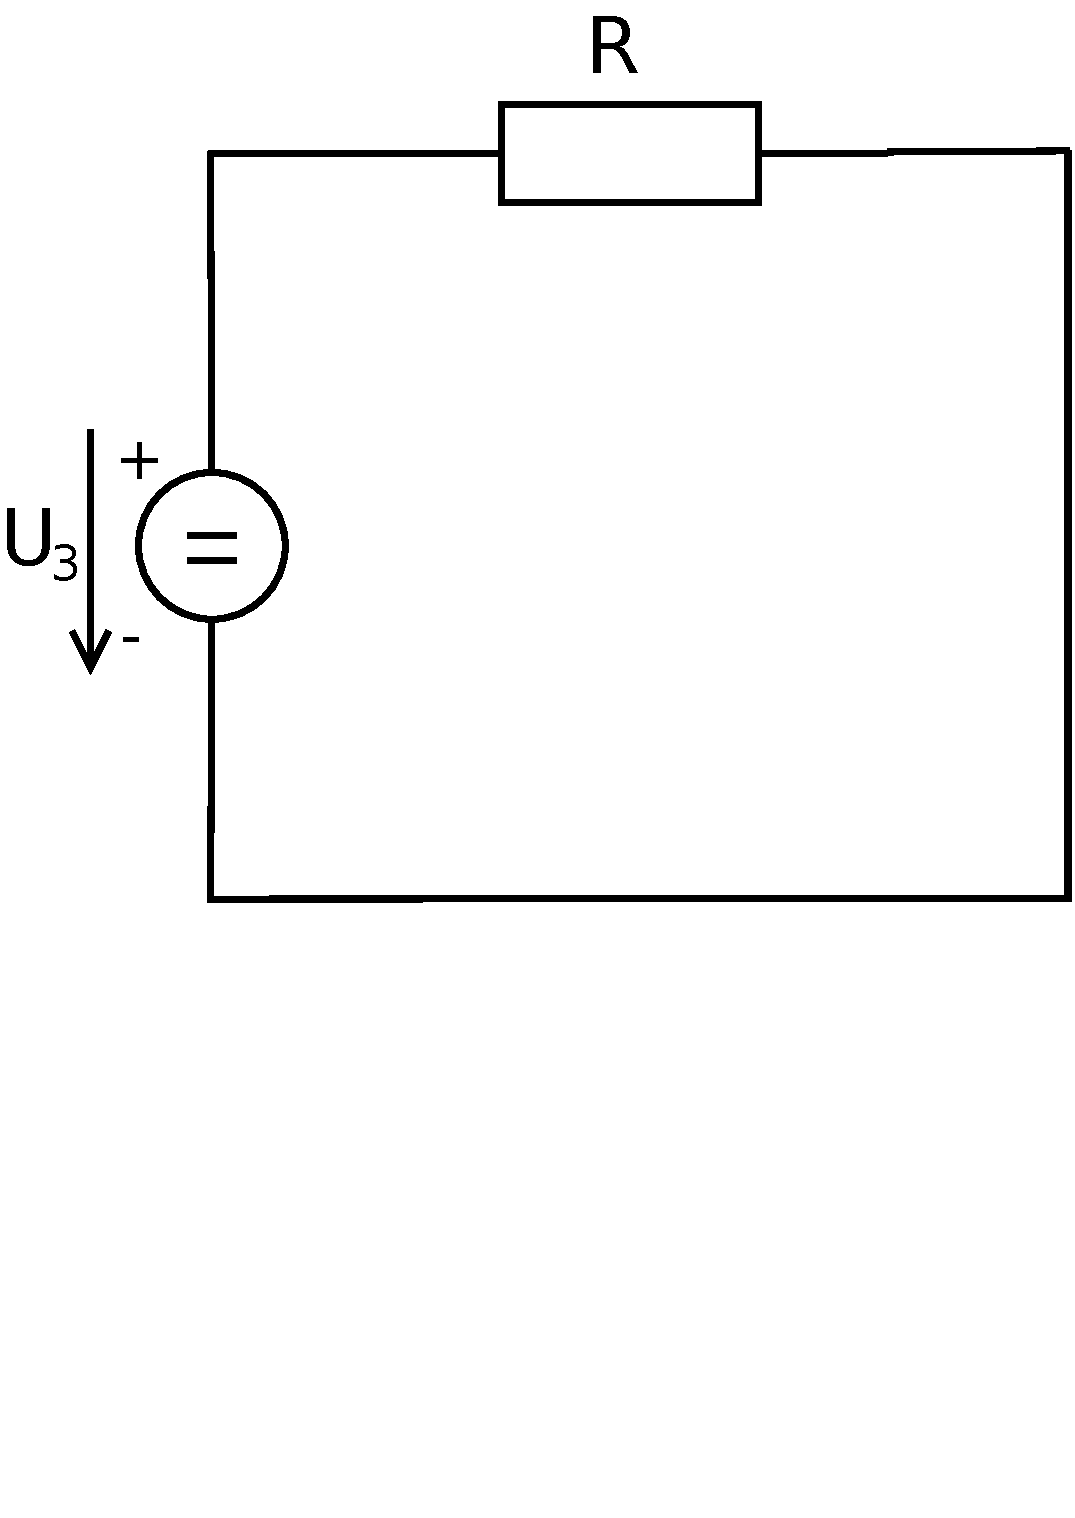
\includegraphics[trim={0 10cm 0 0},clip,width=0.4\linewidth]{obr/1_6}
    \end{figure}
    
    {\Large
        \begin{math}\\
        R = R_A + R_{BC} + R_D = 264,94 + 492,67 + 151,73 = 909,34 {\Omega}\\
        \end{math}
    }
    
    {\Large Vypočítáme proud v obvodu - $U_0$}
    
    {\Large
        \begin{math}\\
        I = \frac{U}{R} = \frac{215}{909,34} = 0,236435216 A\\
        \end{math}
    }
    
    {\Large Dopočítáme napětí a proud}
    
    {\Large
        \begin{math}\\
        U_A = R_A \cdot I = 264,94 \cdot 0,2364 = 62,6411 V\\
        U_D = R_D \cdot I = 151,73 \cdot 0,2364 = 35,8743 V\\
        U_{BC} = U - U_A - U_D = 215 - 62,6411 - 35,8743 = 116,49 V\\
        \\
        I_{5} = \frac{U_{BC}}{R_B} = \frac{116,49}{999,81} = 0,1165 A\\
        U_{5} = I_B \cdot R_5 = 0,1165 \cdot 575 = 66,9945 V\\
        \end{math}
    }
    
    \newpage
    
    %%%%%%%%%%%%%%%%%%%%%%%%%%%%%%%%%%%%%%%%%%%%%%% Příklad 2
    \section*{2. - G \\
    Stanovte napěí UR6 a proud IR6. Použijte metodu Théveninovy věty.}
    
    \begin{tabular}{|c|c|c|c|c|c|c|c|c|} \hline
sk. & $U$ [V] & $R_1$ [$\Omega$] & $R_2$ [$\Omega$] & $R_3$ [$\Omega$] & $R_4$ [$\Omega$] & $R_5$ [$\Omega$] & $R_6$ [$\Omega$] \\ \hline
    {G & 180 & 250 & 315 & 615 & 180 & 460 & 350}{}
    \\ \hline \end{tabular} \\
    
    
    {\Large Vypočítáme vnitřní odpor zdroje - $R_i$ - Théveninova věta}
    
    \begin{figure}[H]
		\vspace{-0.6cm}
		\center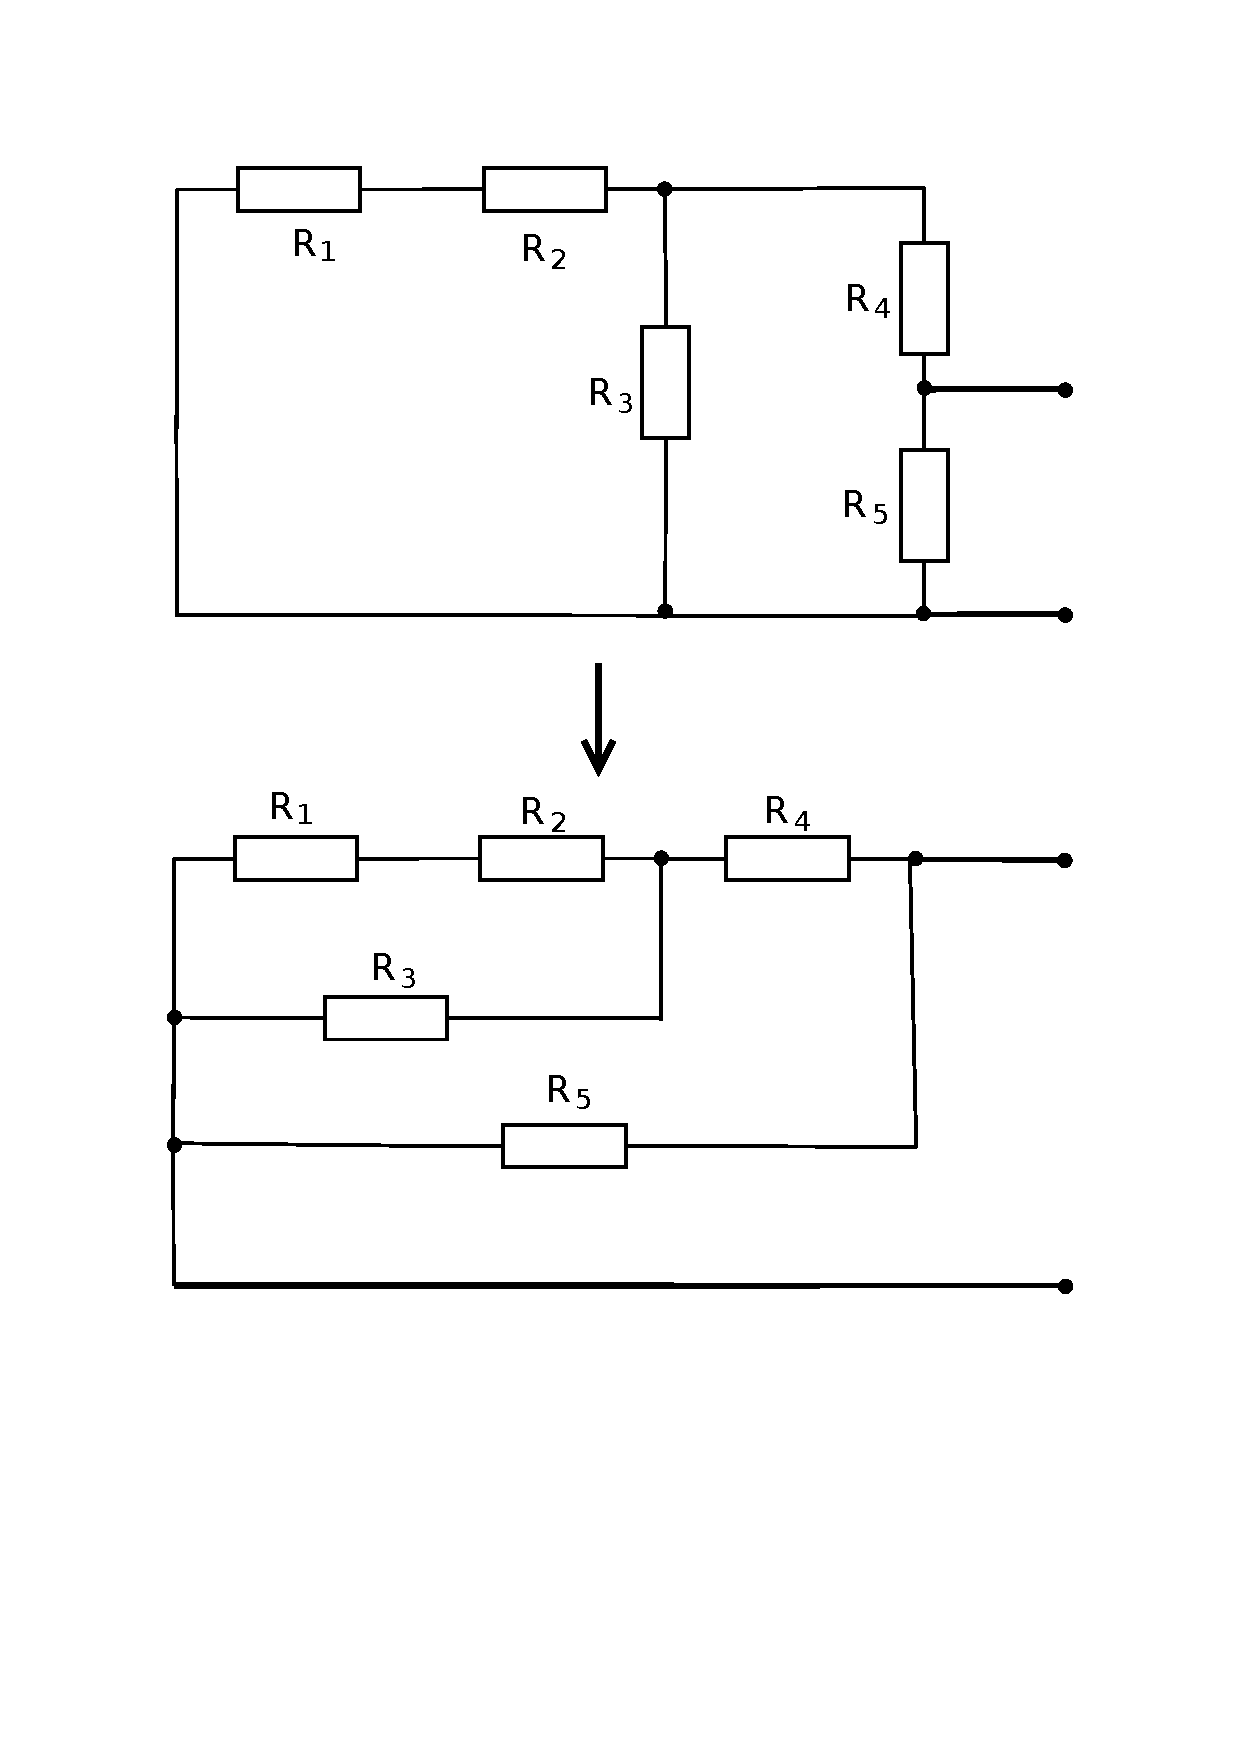
\includegraphics[trim={0 7cm 0 0},clip,width=0.8\linewidth]{obr/2_2}
		\caption*{Představíme si obvod z pohledu svorek.}
    \end{figure}
    
    {\Large
        \begin{math}\\
        R_{12} = R_1 + R_2 = 250 + 315 = 565 {\Omega}\\
        R_{123} = \frac{R_{12} \cdot R_3}{R_{12} + R_3} = \frac{565 \cdot 615}{565 + 615} = \frac{347475}{1180} = 294,47033 {\Omega}\\
        R_{1234} = R_{123} + R_4 = 294,47033 + 180 = 474,47033 {\Omega}\\
        R_i = \frac{R_{1234} \cdot R_5}{R_{1234} + R_5} = \frac{474,47033 \cdot 460}{474,47033 + 460} = \frac{218256,3518}{934,47033} = 233,56156{\Omega}\\
        \end{math}
    }
    
    {\Large Vypočítáme napětí zdroje - $U_0$ - Metodou postupného zjednodušování (bez zátěže)}
    
    \begin{figure}[H] 
		\vspace{-0.6cm}
		\center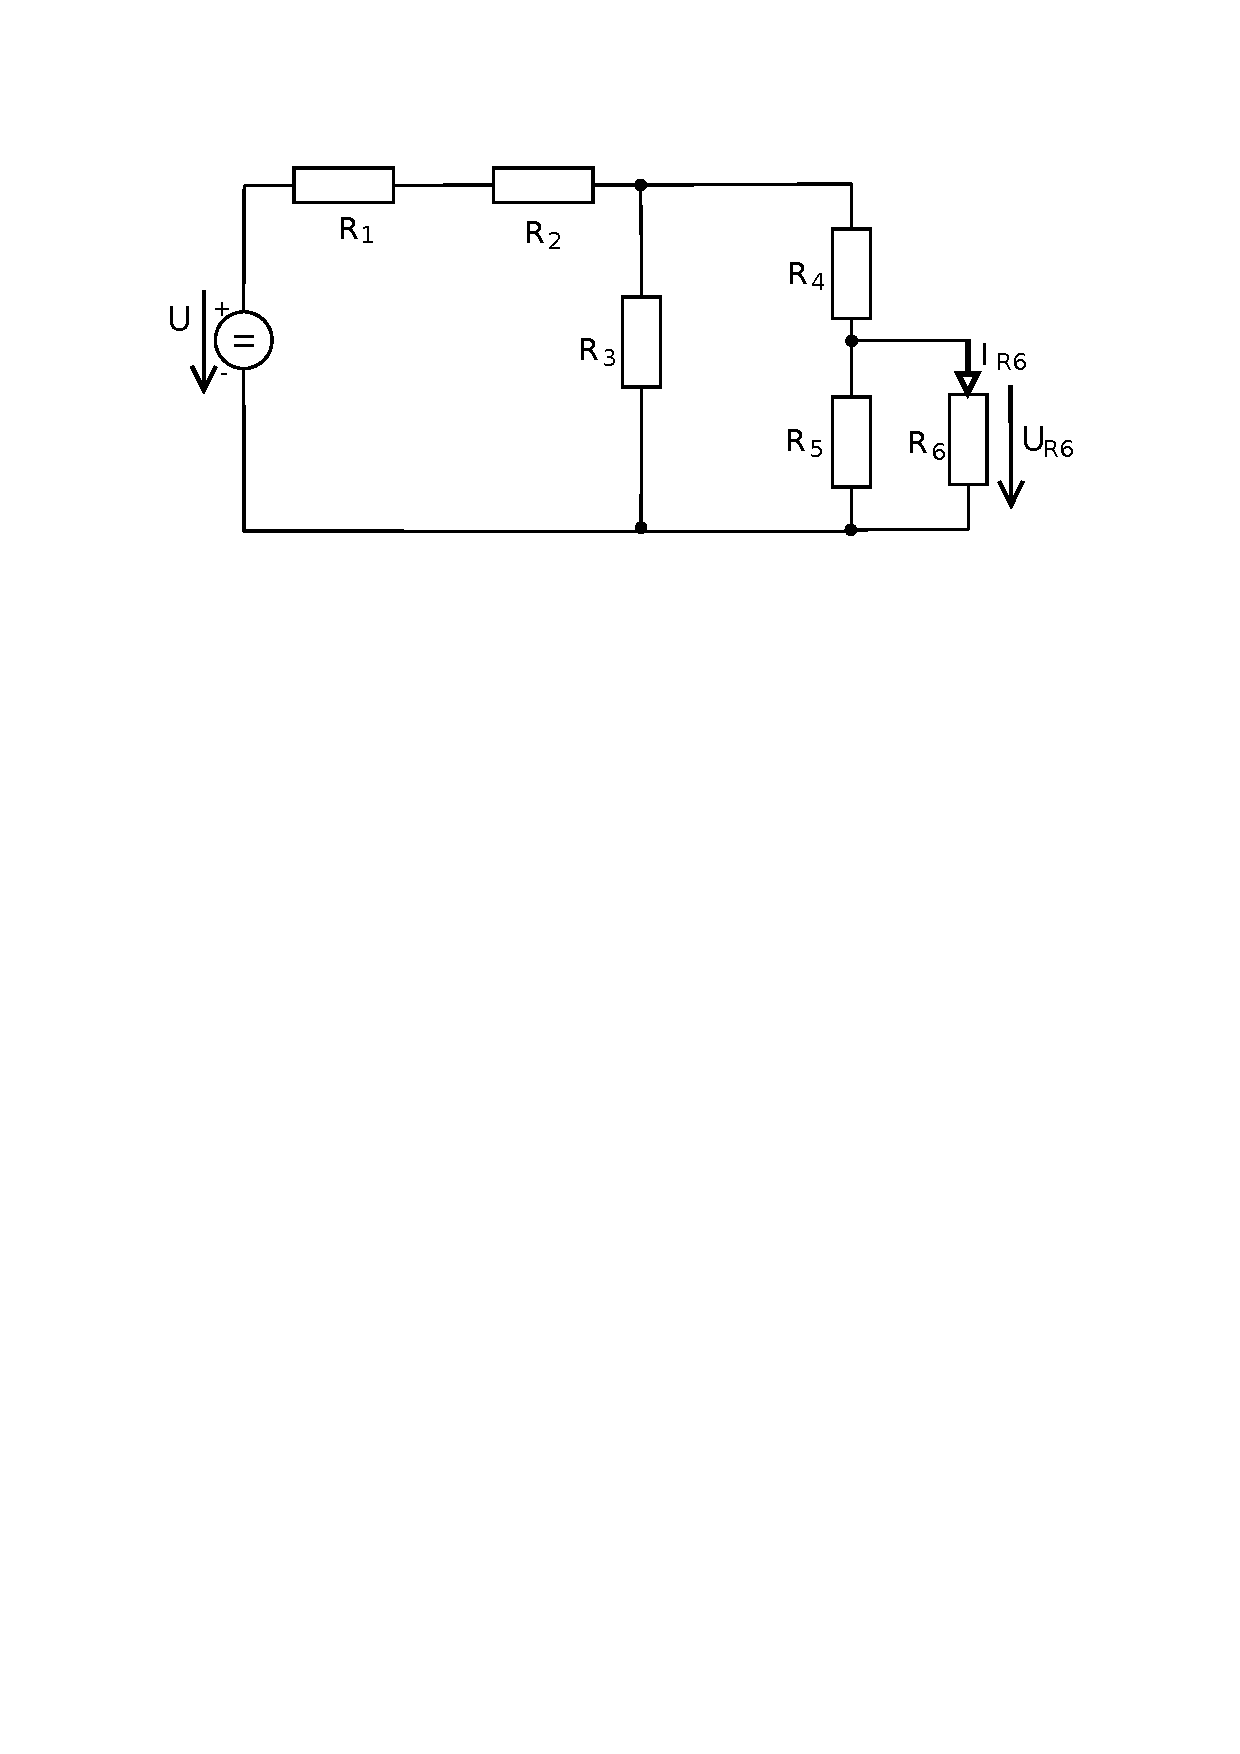
\includegraphics[trim={0 20cm 0 0},clip,width=0.9\linewidth]{obr/2_1}
		\caption*{Zadání}
    \end{figure}
    
    \begin{figure}[H] 
		\vspace{-0.6cm}
		\center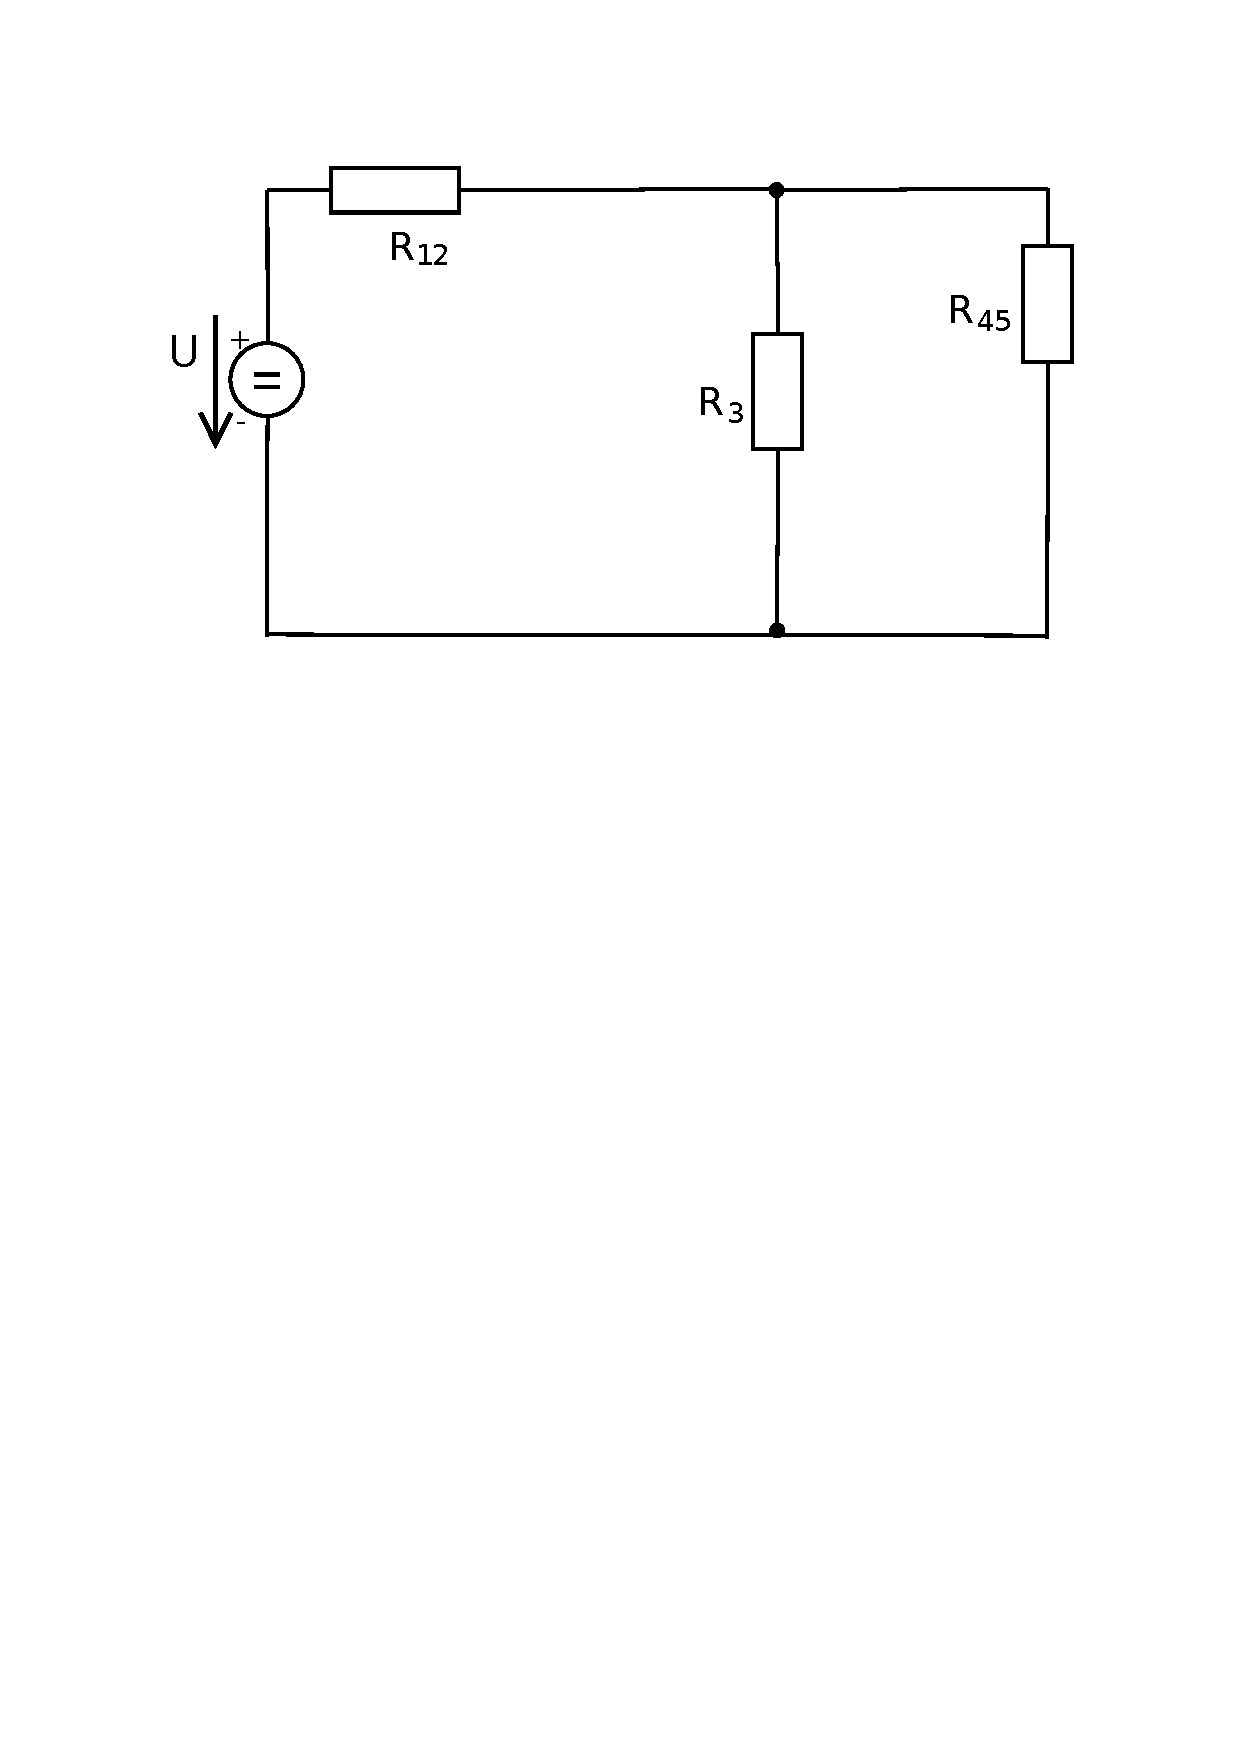
\includegraphics[trim={0 17cm 0 0},clip,width=0.7\linewidth]{obr/2_3}
    \end{figure}
    
    {\Large
        \begin{math}\\
        R_{12} = R_1 + R_2 = 250 + 315 = 565 {\Omega}\\
        R_{45} = R_4 + R_5 = 180 + 460 = 640 {\Omega}\\
        \end{math}
    }
    
    \begin{figure}[H] 
		\vspace{-0.6cm}
		\center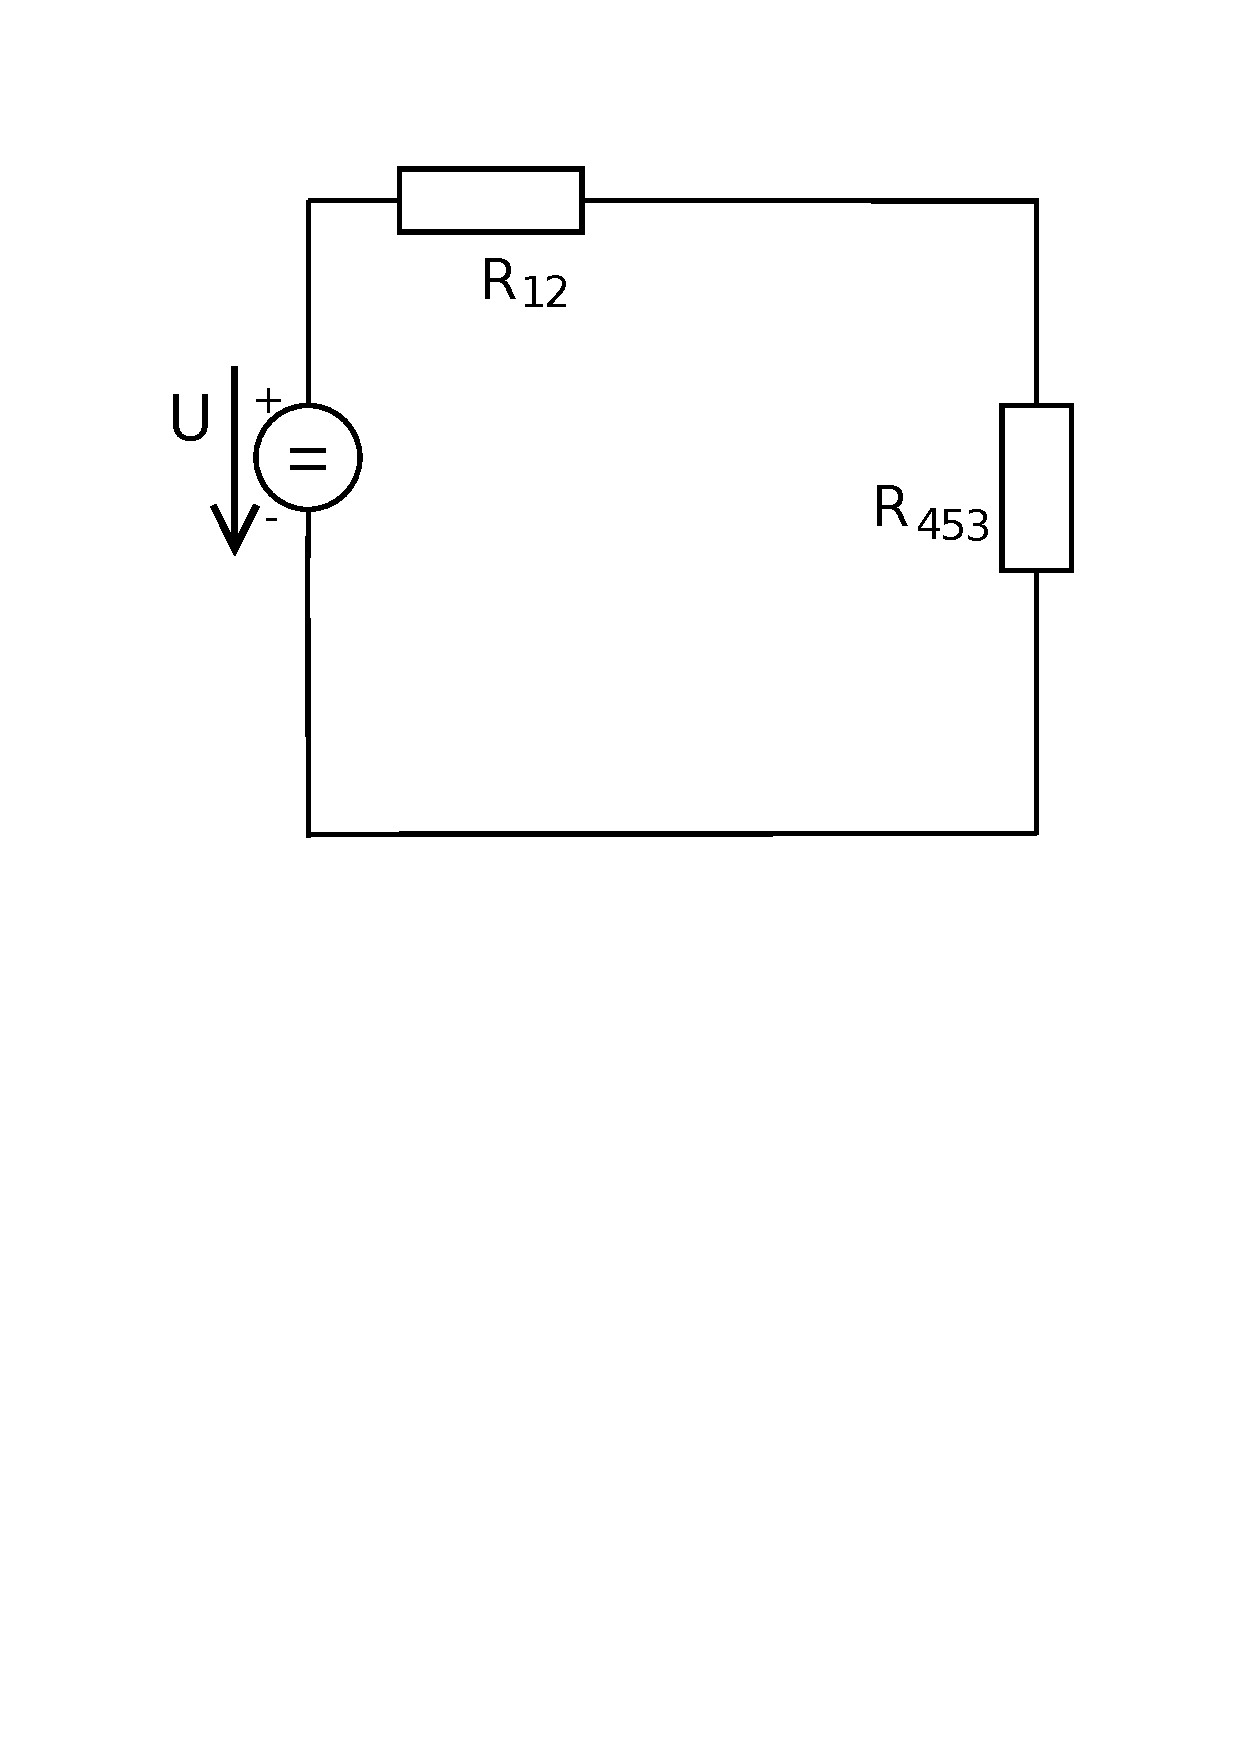
\includegraphics[trim={0 13cm 0 0},clip,width=0.5\linewidth]{obr/2_4}
    \end{figure}
    
    {\Large
        \begin{math}\\
        R_{453} = \frac{R_{45} \cdot R_3}{R_{45} + R_3} = \frac{640 \cdot 615}{640 + 615} = \frac{393600}{1255} = 313,62549 {\Omega}\\
        \end{math}
    }
    
    \begin{figure}[H] 
		\vspace{-0.6cm}
		\center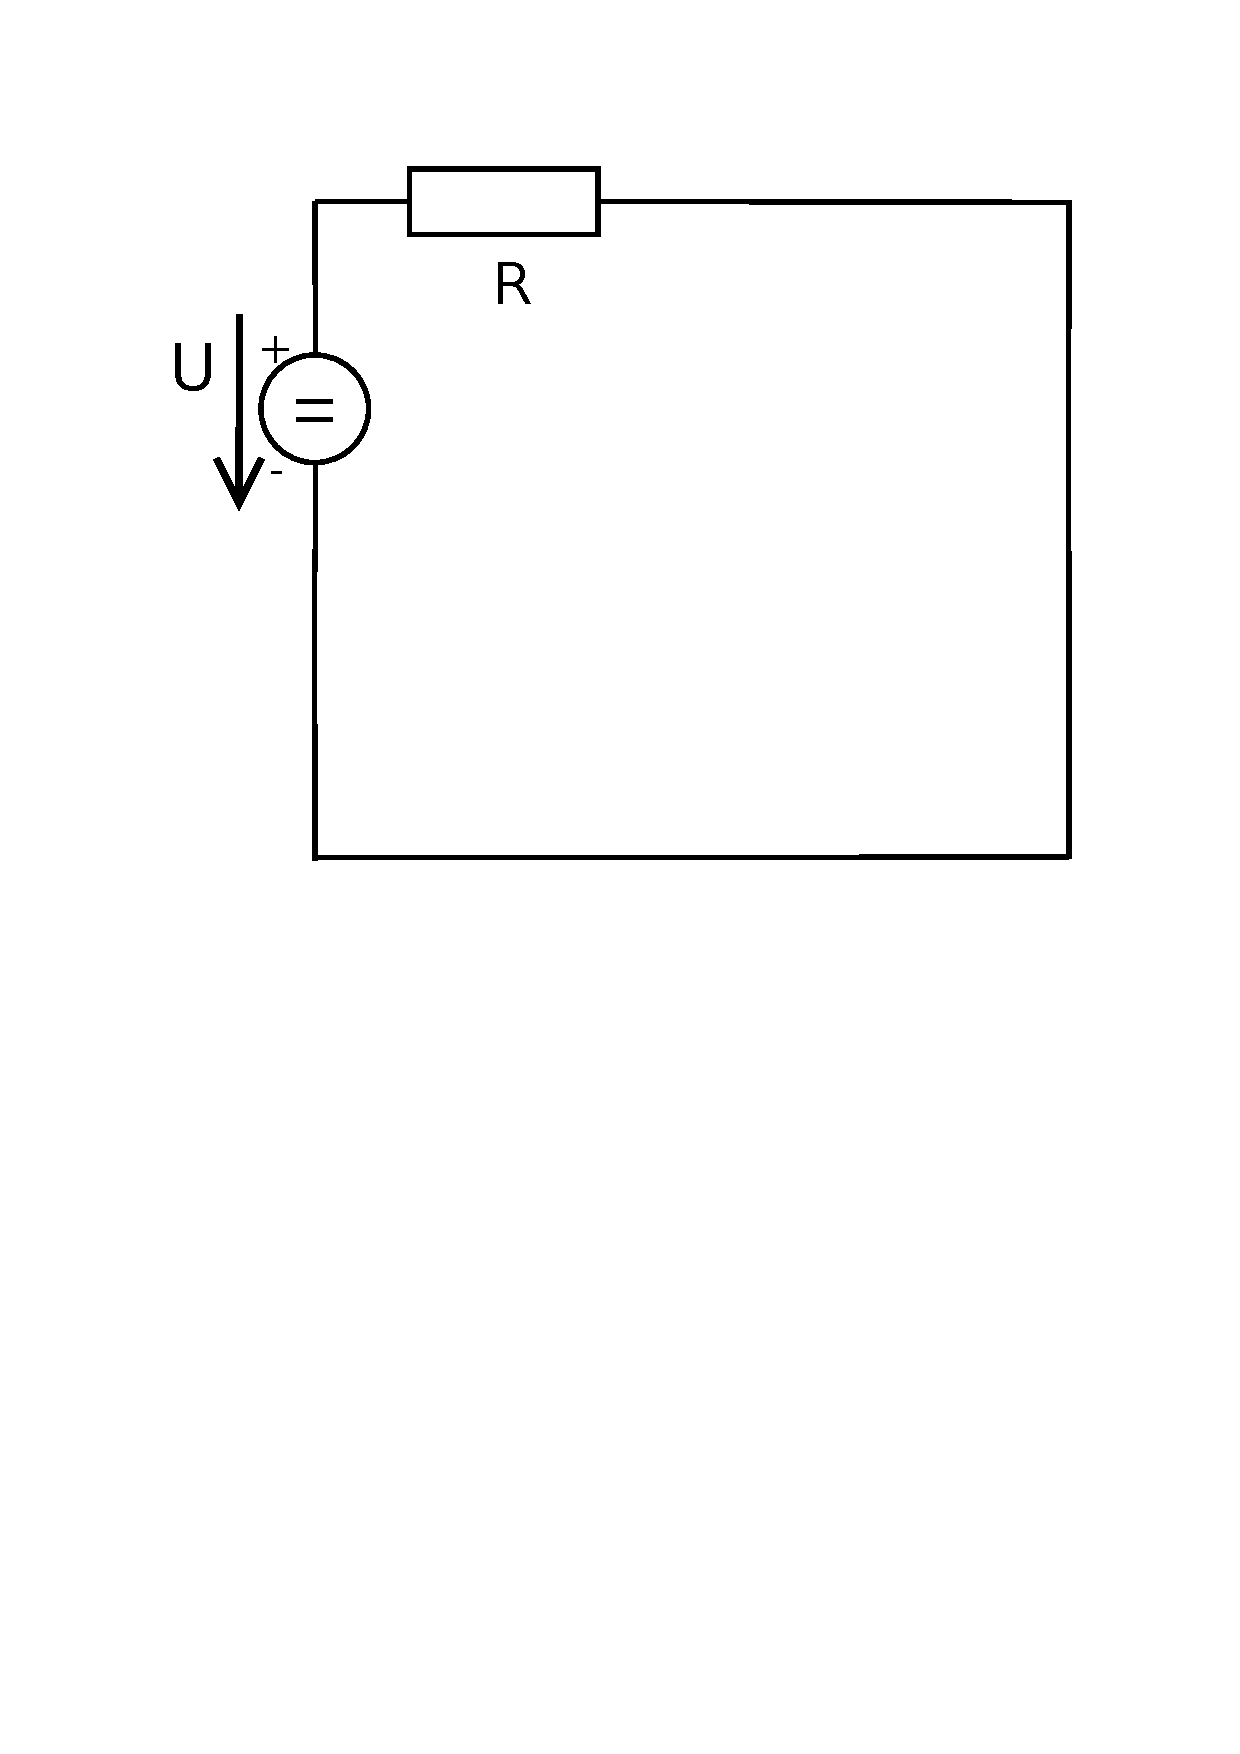
\includegraphics[trim={0 12cm 0 0},clip,width=0.5\linewidth]{obr/2_5}
    \end{figure}
    
    {\Large
        \begin{math}\\
        R = R_{12} + R_{453} = 565 + 313,62549 = 878,62549 {\Omega}\\
        \\
        \\
        I = \frac{U}{R} = \frac{180}{878,62549} = 0,204865 A\\
        U_{453} = R_{453} \cdot I = 313,62549 \cdot 0,204865 = 64,25088 V\\
        I_{45} = \frac{U_{453}}{R_{45}} = \frac{64,25088}{640} = 0,100392 A\\
        U_0 = U_5 = R_5 \cdot I_45 = 460 \cdot 0,100392 = 46,18032 V\\
        \end{math}
    }
\newpage
    {\Large Přičteme zátěž - $R_6$}
    
    \begin{figure}[H] 
		\vspace{-0.6cm}
		\center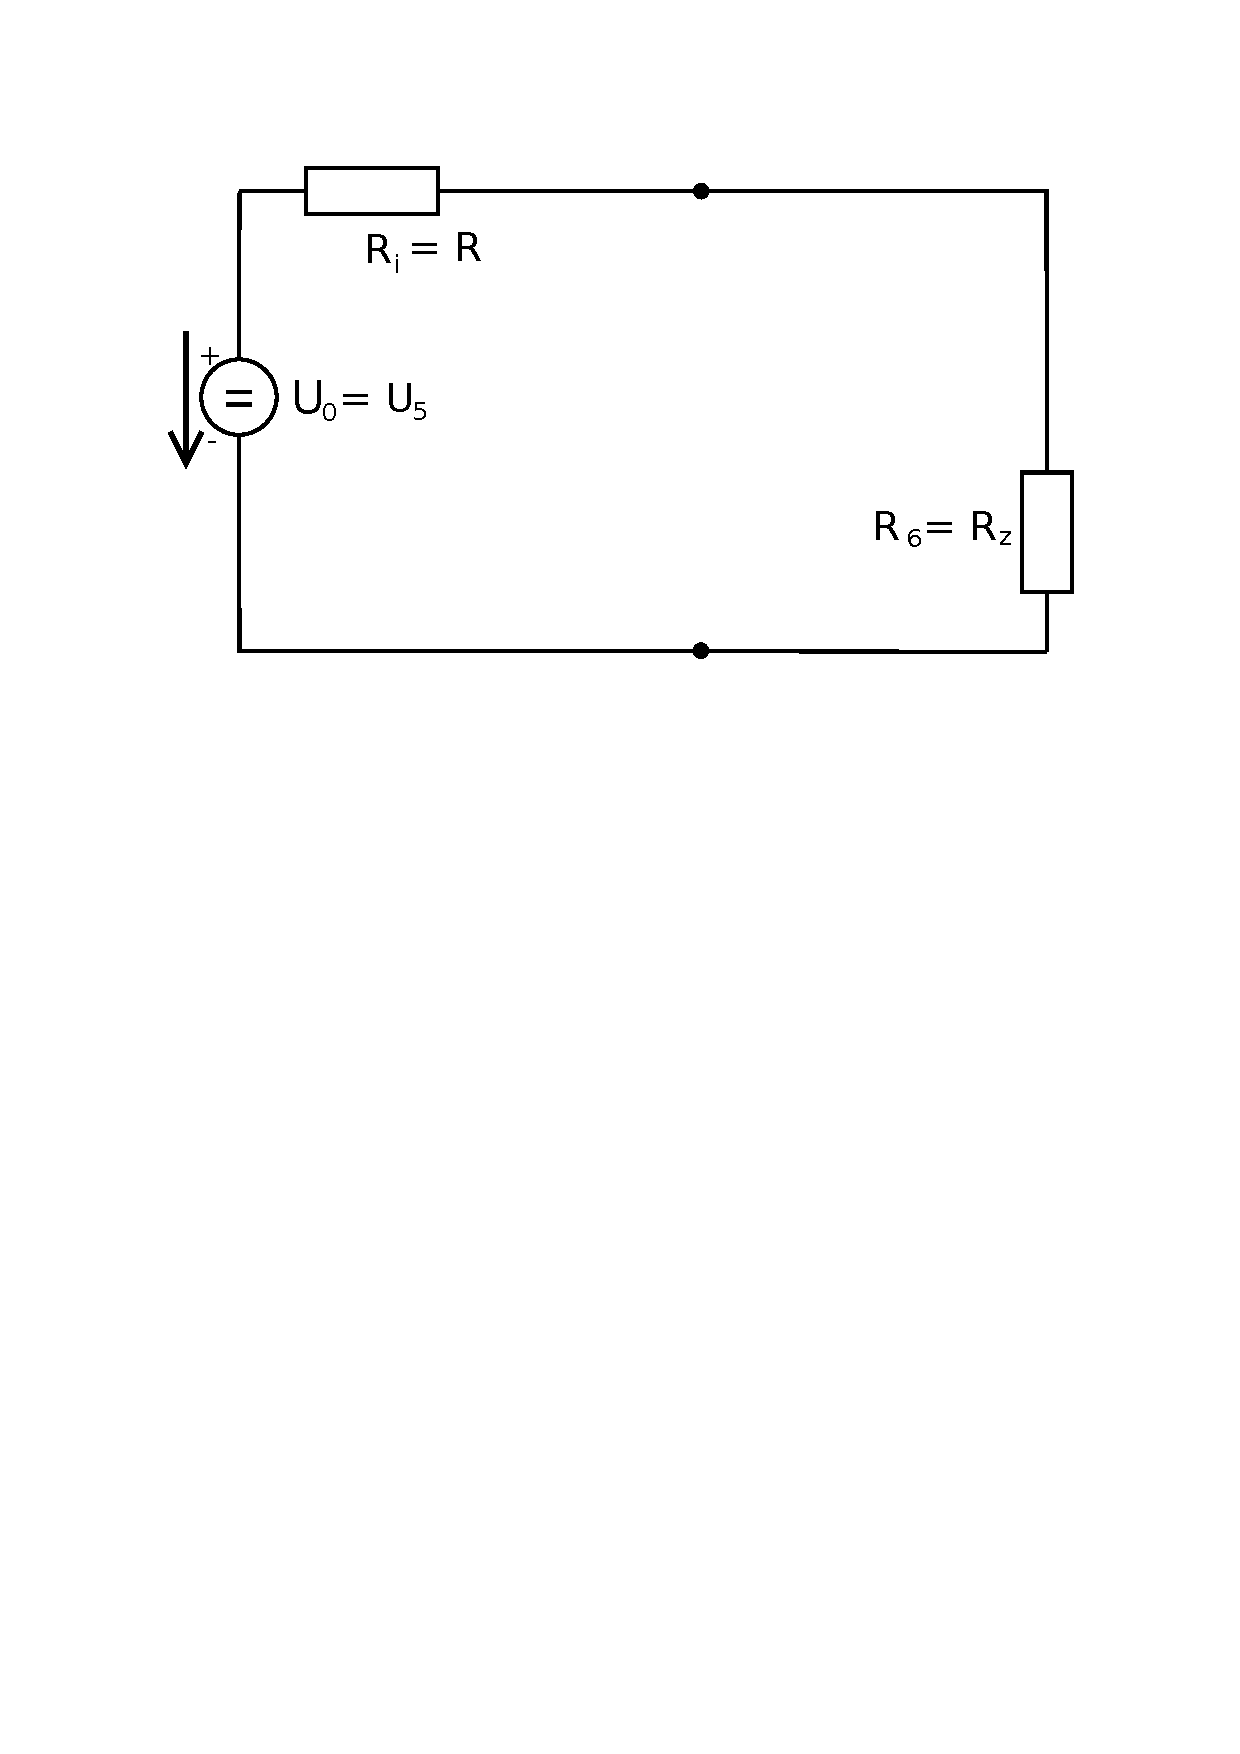
\includegraphics[trim={0 18cm 0 0},clip,width=0.8\linewidth]{obr/2_6}
    \end{figure}
    
    {\Large
        \begin{math}\\
        R_{i6} = R_i + R_6 = 233,56156 + 350 = 583,56156 {\Omega}\\
        \end{math}
    }
    
    {\Large Dopočítáme napětí a proud - $U_{R6}$ a $I_{R6}$}
    
    {\Large
        \begin{math}\\
        I_{R6} = I = \frac{U_5}{R_{i6}} = \frac{46,18032}{583,56156} = 0,791353 A\\
        U_{R6} = I_{R6} \cdot R_6 = 0,791353 \cdot 350 = 27,697358 V\\
        \end{math}
    }
    
    \newpage
    
\section{Shrnutí výsledků}
    \begin{tabular}{|c|c|c|} \hline 
        \textbf{Příklad} & \textbf{Skupina} & \textbf{Výsledky} \\ \hline
        1 & \prvniSkupina & $U_{R5} = $ 66,9945 V \qquad \qquad $I_{R5} = $ 0,1165 A \\ \hline
        2 & \druhySkupina & $U_{R6} = $ 27,6974 V \qquad \qquad $I_{R6} = $ 0,7914 A\\ \hline
        3 & \tretiSkupina & $U_{R4} = $ \qquad \qquad $I_{R4} = $\\ \hline
        4 & \ctvrtySkupina & $|U_{C_{2}}| = $ \qquad \qquad $\varphi_{C_{2}} = $ \\ \hline
        5 & \patySkupina & $u_C = $ \\ \hline
    \end{tabular}
\end{document}